\documentclass[letterpaper]{article} % DO NOT CHANGE THIS
\usepackage[submission]{aaai2027} % DO NOT CHANGE THIS
\usepackage[hyphens]{url} % DO NOT CHANGE THIS
\usepackage{graphicx} % DO NOT CHANGE THIS
\urlstyle{rm} % DO NOT CHANGE THIS
\def\UrlFont{\rm} % DO NOT CHANGE THIS
\usepackage{natbib} % DO NOT CHANGE THIS AND DO NOT ADD OPTIONS
\usepackage{caption} % DO NOT CHANGE THIS AND DO NOT ADD OPTIONS
\frenchspacing % DO NOT CHANGE THIS

\usepackage{booktabs}
\usepackage{amsmath}
\usepackage{amssymb}
\usepackage{CJKutf8}
\makeatletter
\expandafter\let\csname ver@CJK.sty\endcsname\relax
\makeatother

\pdfinfo{
/TemplateVersion (2027.1)
}

\setcounter{secnumdepth}{2}

\title{\begin{CJK*}{UTF8}{gbsn}超越权重几何：以域条件功能谱追踪 On-Policy Distillation\\补充材料\end{CJK*}}
\author{Anonymous Submission}
\affiliations{}

\begin{document}
\maketitle
\begin{CJK*}{UTF8}{gbsn}
\appendix

\section{数学基础}

\subsection{白化坐标表示同一权重映射}

固定一个 checkpoint、输入域和线性模块，记
\begin{equation}
\Sigma=\mathbb E[hh^\top],\qquad S=\Sigma^{1/2},\qquad A=WS,
\end{equation}
其中 $S$ 是对称半正定平方根，$S^\dagger$ 是 Moore--Penrose 伪逆。令
$z=S^\dagger h$，$P=S^\dagger S$ 为 $\operatorname{range}(\Sigma)$ 上的正交投影。
对任意 $v\in\ker(\Sigma)$，有
$\mathbb E[(v^\top h)^2]=v^\top\Sigma v=0$，因此 $h$ 几乎处处位于
$\operatorname{range}(S)$。于是
\begin{equation}
h=Sz,\qquad \mathbb E[zz^\top]=P,\qquad Wh=WSz.
\label{eq:supp-whiten}
\end{equation}
在 $\Sigma$ 的支撑空间内，$P$ 就是恒等映射。因而 $WS$ 不是额外构造的激活模型，
而是原权重映射在域条件白化输入坐标中的表示。

\subsection{输出二阶矩与最优近似}

对模块输出 $y=Wh$，
\begin{equation}
AA^\top=W\Sigma W^\top=\mathbb E[yy^\top].
\label{eq:supp-output}
\end{equation}
所以 $\sigma_i^2(A)$ 是模块输出二阶矩的第 $i$ 个特征值，且
$\|A\|_F^2=\mathbb E\|y\|_2^2$。对任意候选权重 $\widetilde W$，
\begin{equation}
\mathbb E\|(W-\widetilde W)h\|_2^2
=\|(W-\widetilde W)S\|_F^2.
\label{eq:supp-error}
\end{equation}
令 $A_r$ 为 $A$ 的 rank-$r$ 截断 SVD。由于 $A=WS$ 的非零右奇异方向位于
$\operatorname{range}(S)$，取 $\widetilde W_r=A_rS^\dagger$ 即有
$\widetilde W_rS=A_r$。由 Eckart--Young--Mirsky 定理，
\begin{equation}
\min_{\operatorname{rank}(\widetilde W)\le r}
\mathbb E\|(W-\widetilde W)h\|_2^2
=\sum_{i>r}\sigma_i^2(A).
\label{eq:supp-optimal}
\end{equation}
因此，$r_\varepsilon(WS)$ 是使最优近似损失不超过模块期望输出能量
$\varepsilon$ 比例的最小秩。

\subsection{输入坐标重参数化不变性}

对可逆输入坐标变换 $h'=Th$，令
$W'=WT^{-1}$、$\Sigma'=T\Sigma T^\top$，并令 $S'$ 为 $\Sigma'$ 的任一平方根，则
\begin{equation}
(W'S')(W'S')^\top
=W'\Sigma'(W')^\top
=W\Sigma W^\top.
\end{equation}
所以 $W'S'$ 与 $WS$ 的非零奇异值相同。可逆缩放能够改变裸权重谱，却不改变功能谱；
这正是正文所说的坐标尺度修正。

\subsection{Current、Fixed 与 Centered 输入度量}

主构念使用当前二阶矩 $W_tS_{D,t}$；fixed whitening 使用
$W_tS_{D,0}$，把所有 checkpoint 放在 base 输入度量上。恒等式
\begin{equation}
W_tS_t-W_0S_0
=(W_t-W_0)S_0+W_t(S_t-S_0)
\label{eq:supp-fixed}
\end{equation}
并不是因果分解：$S_t$ 是当前模型前层计算的内生结果，且 $r_\varepsilon$ 是非线性的。
因此 fixed whitening 只能检查对输入度量更新的敏感性，不能解释为“激活造成了多少压缩”。

Centered 审计把 $\Sigma$ 替换为
\begin{equation}
\Sigma^{\mathrm c}
=\mathbb E[(h-\mathbb E h)(h-\mathbb E h)^\top].
\end{equation}
它删除激活均值方向，使被估计量从输出二阶矩变为输出协方差。本文将其作为边界检查，
不以其替代正文定义。

\subsection{离散秩与连续谱稳定性}

若 $\widetilde A=A+E$，Weyl 不等式给出
$|\sigma_i(\widetilde A)-\sigma_i(A)|\le\|E\|_2$。当累计能量阈值与相邻交点有余量时，
离散 $r_\varepsilon$ 对小扰动稳定；在平坦谱段上则可能移动少量方向。因此我们同时检查
$\varepsilon\in\{.01,.025,.05,.10\}$ 以及
\begin{align}
r_{\mathrm{stable}}(A)&=\frac{\|A\|_F^2}{\|A\|_2^2},\\
r_{\mathrm{ent}}(A)&=\exp\left(-\sum_i p_i\log p_i\right),
\quad p_i=\frac{\sigma_i^2}{\sum_j\sigma_j^2}.
\end{align}
两个连续量用于判断训练设置排序是否只是单一阈值造成的。

\section{实验与估计协议}

\subsection{训练设置与 checkpoint 交集}

两条学生轨分别为 Qwen3-4B-Base 和 Llama-3.2-3B，所有训练设置均使用 rank-32 LoRA。
OPD 在 current-student rollout 上使用 teacher forward KL；off-KD 在冻结 teacher 序列上
使用相同软目标；seqKD 严格复用 off-KD 的序列、顺序与步数，只将目标改为 hard next-token CE；
SFT 使用外部 reference CoT。Qwen 另有 $\alpha=.5$ current-self exposure，
Llama 另有 frozenSelf0-KD，后者永久复用 step-0 student 生成的 rollout。

\begin{table}[t]
\centering
\small
\setlength{\tabcolsep}{3.5pt}
\begin{tabular}{lccc}
\toprule
训练设置 & 序列生产者 & 刷新 & 监督目标 \\
\midrule
OPD & current student & 是 & teacher KL \\
$\alpha=.5$ & mixed support & 是 & teacher KL \\
frozenSelf0 & step-0 student & 否 & teacher KL \\
off-KD & teacher & 否 & teacher KL \\
seqKD & teacher & 否 & hard CE \\
SFT & external reference & 否 & hard CE \\
\bottomrule
\end{tabular}
\caption{各训练设置所控制的变量。辅助设置并非在两个模型上都存在；主比较只使用严格
checkpoint 交集，不对缺失 checkpoint 插值。}
\label{tab:supp-arms}
\end{table}

双模型共同早期窗口为 step 20、40、80，轨迹积分的共同 horizon 为 step 320。
FAT 输出分析每个域包含 Llama 的 6 个非零 checkpoint 和 Qwen 的 9 个非零 checkpoint。
checkpoint-held-out fold 将同一 checkpoint 的四种训练设置整体放入同一 fold。

\subsection{输入域、样本与 mask}

四个核心几何 probe 是冻结的 general text、32 条 held-out Hendrycks MATH、
MMLU-Pro 和 IFEval。Llama 分别使用 128、32、128 和 541 个样本。冻结文本、sample ID、
tokenization、文本 hash 与 token mask 共同定义输入域；动态训练 rollout 不会替代这些外部 probe。

FAT 使用完整 MMLU-Pro 1,400 题和 MATH500 500 题。所有 checkpoint 在完全相同的
固定参考序列上 teacher forcing。MMLU-Pro 划分为 prompt $P$、正确标签前格式 $F$、
正确 answer-choice label $A$ 与 termination $T$；MATH 划分为 prompt $P$、最终 boxed answer 前推理 $C$、
token-clean boxed answer $B$ 与 termination $T$。区域 mask 后先逐样本计算完整词表
$D_{\mathrm{KL}}(p_0\Vert p_t)$ 和 reference-token NLL，再对样本 macro 平均。

Math $C$ 使用数据集参考解答中、最终 boxed-answer span 之前的 token-clean 推理区域。
该补充计算覆盖 62 个 model states 和 31,000 条 sample rows；每个 state 使用全部 500 题，
BF16 forward 后以 FP32 \texttt{log\_softmax} 计算 KL，先在每题的 $C$ tokens 内平均，再对题目
macro 平均。Box 边界不闭合或 tokenizer span 无法唯一确定时按冻结规则登记，而不事后移动边界。

\subsection{功能谱计算}

每个基本单元由模型、训练设置、checkpoint、域、层和模块六个索引共同确定。
每个样本先在自己的有效 token/window 内归一化二阶矩，再对样本等权。七类模块为
q/k/v/o 与 gate/up/down。所有相对变化都先在模块内计算，再进行聚合，避免矩阵尺寸决定层级摘要。
正文 equal-5 使用 v/o/gate/up/down；q/k 与 equal-7 见 Sec.~C.2。

两条轨均读取序列化 BF16 deployed merged checkpoint，使用 BF16 forward、FP32 构造
$WS$，并以 FP64 完成 SVD/rank accumulation。Llama 以 FP32 累积 Gram，再以 FP64
进行对称特征分解；Qwen 审计 manifest 将 Gram/whitening 记录为 FP64。由舍入导致的负小特征值
截断为零，不添加 jitter。独立 matched 数值轨在共同单元上得到
Spearman $.9966$、MAE $.00050$。

\subsection{权重与激活基线}

对 centered hidden-state covariance 的特征值 $\lambda_i$，令
$q_i=\lambda_i/\sum_j\lambda_j$。纯激活组包含
\begin{equation}
\mathrm{ER}=\exp\!\left(-\sum_iq_i\log q_i\right),\qquad
\mathrm{PR}=\frac{(\sum_i\lambda_i)^2}{\sum_i\lambda_i^2},
\end{equation}
top-1/8/32 variance share、raw/centered anisotropy，以及相对同 probe step 0 的
linear CKA。严格共同网格中的 $A$ 正是这八项特征。

TPNT 先以 source top-$k$ SVD 重建 $W_0^{(k)}$，取其绝对值最大的 $\alpha$ 比例坐标
$M_{\mathrm{princ}}$，并报告
\begin{equation}
\begin{aligned}
\mathrm{OverlapLift}_{k,\alpha}
&=\frac{|M_{\mathrm{princ}}\cap M_\Delta|}{\alpha|M_\Delta|},\\
M_\Delta&=\mathbf1[\Delta W\ne0].
\end{aligned}
\end{equation}
正式审计同时减去 spectrum-matched random-subspace null。PABS 则以
$q_i^U=\sigma_i(U_{0,k}^\top U_{t,k})$ 和
$q_i^V=\sigma_i(V_{0,k}^\top V_{t,k})$ 定义
\begin{equation}
\mathrm{PABS}_k=\frac{1}{2k}\sum_i(q_i^U+q_i^V).
\end{equation}
NSS 比较两端各自归一化的 top-32 奇异值谱。强权重位置基线为
source-principal joint projection：
\begin{equation}
p_k=\frac{\|U_k^\top\Delta W V_k\|_F^2}{\|\Delta W\|_F^2},
\qquad k\in\{4,8,16,32\}.
\end{equation}
公平比较时，$p_k$ 与功能压缩使用相同的五模块和完全相同的 checkpoint 状态。
Teacher KL 的 top-32 近似在 Qwen off-KD、Llama off-KD 与 Llama frozenSelf0-KD
上的 token-weighted retained mass 分别为 $.999987$、$.999212$、$.998134$。

\subsection{统计协议}

逐臂 Spearman 把 checkpoint 当作有序观测，描述单条轨迹上的单调共变，不把它们当成独立重复。
Checkpoint demeaning 在 model--domain--checkpoint 内先减去四设置同期均值，再 pooled 计算相关。
预测比较按完整 checkpoint group 留出；标准化和 ridge 选择都只在训练 fold 内完成。
成对读出分析按 checkpoint group 或 paired item 进行 bootstrap。由于每种训练设置只有一个独立 seed，
这些区间都不代表跨 seed 的训练不确定性。

\section{功能轨迹结果与稳健性}

\subsection{完整域轨迹}

图 \ref{fig:supp-full} 将正文均值轨迹展开到四个核心域。在 $\varepsilon=.05$ 下，
OPD 在 24 个双模型早期 model--domain--checkpoint 单元中均为 equal-5 压缩最深。
扩展到四个阈值后，Llama 的 48 个单元全部成立，Qwen 为 47 个成立；唯一例外是
Qwen IFEval、step 20、$\varepsilon=.10$，连续 margin 为 $-0.8$ direction。
这支持共同的早期排序，不支持完全相同的时间形态或普遍终点规律。

\begin{figure*}[t]
\centering
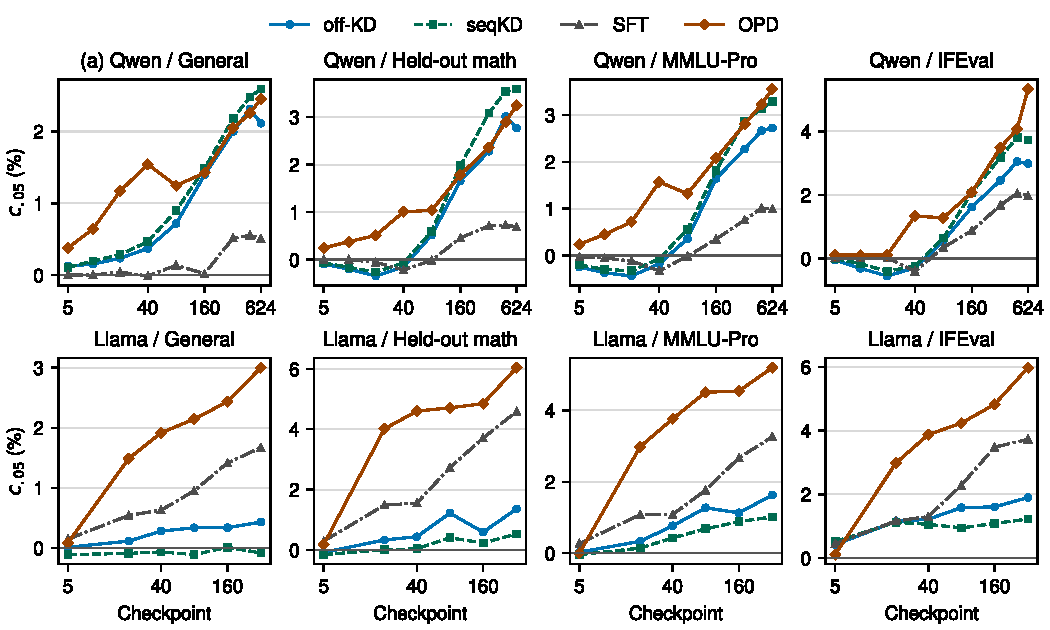
\includegraphics[width=\textwidth]{figures/supp_fig_full_domain_trajectories.pdf}
\caption{Qwen 与 Llama 在四个冻结输入域上的完整 equal-5 轨迹。各 panel 保留原始
checkpoint 网格，不使用平滑或插值。}
\label{fig:supp-full}
\end{figure*}

\subsection{为什么正文使用 Equal-5、Equal-7 仍需审计}

Query/key 共同形成 attention score，更接近注意力路由；value/output 与 MLP projection
更直接变换所承载的内容。更关键的是，逐模块审计发现 q/k 的训练设置排序异质，且基线功能秩较小：
少量方向变化就会在相对平均中获得较大权重。排除 q/k 不是声称它们无关。

\begin{table}[t]
\centering
\small
\setlength{\tabcolsep}{4pt}
\begin{tabular}{lrr}
\toprule
范围 & q+k 原始 rank 占比 & 相对压缩占比 \\
\midrule
Qwen & 12.5\% & 46.4\% \\
Llama & 5.8\% & 25.8\% \\
双模型 & 7.7\% & 32.2\% \\
\bottomrule
\end{tabular}
\caption{$\varepsilon=.05$ 时 q/k 在早期 OPD 压缩中的占比。第一列计算减少的方向数，
第二列先按各模块基线秩归一化；两者都不是因果贡献或输出能量占比。}
\label{tab:supp-qk}
\end{table}

在 $\varepsilon=.01,.025,.05,.10$ 下，q+k 的原始 rank-count 占比分别为
$17.1\%,11.9\%,7.7\%,3.2\%$，相对压缩占比分别为
$35.8\%,33.8\%,32.2\%,27.4\%$。因此 q/k 的绝对方向数贡献较少，尤其在 Llama 中；
但相对自身基线的变化并不小。Equal-7 仍保留总体趋势，却会因这种异质性削弱跨模型 OPD dominance。

\subsection{阈值、连续秩、中心化与层级审计}

\begin{figure*}[t]
\centering
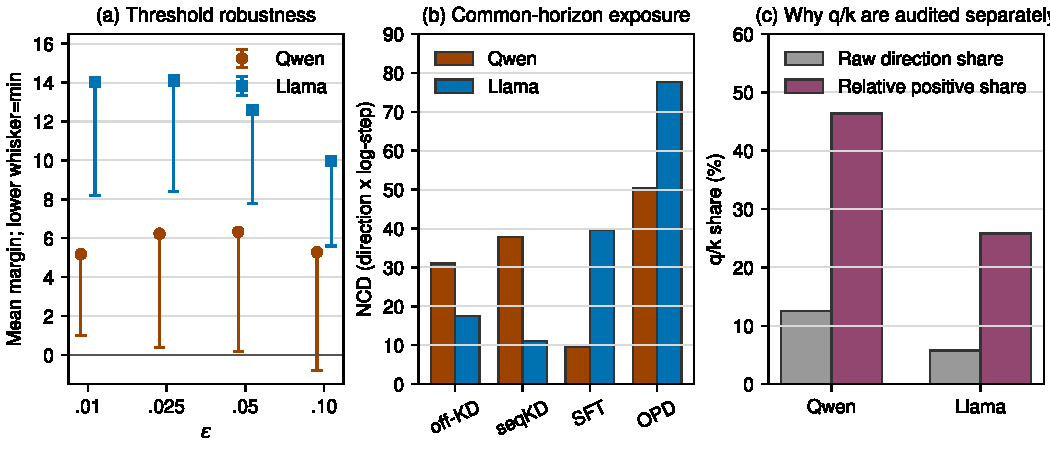
\includegraphics[width=\textwidth]{figures/supp_fig_robustness.pdf}
\caption{Llama 早期排序的稳健性。Threshold rank、stable rank、entropy effective rank
及 centered covariance 均在 equal-5 聚合中保留更深的 OPD 压缩；异质的 q/k 单独展示。}
\label{fig:supp-robust}
\end{figure*}

Llama 在 $r_{.05}$、stable rank 与 entropy effective rank 的每个早期
model--domain--checkpoint 单元中都由 OPD 压缩最深。OPD/SFT/off-KD/seqKD 的早期平均变化分别为
$16.214/6.464/3.976/2.333$ directions、
$.376/.165/.061/.029$ stable-rank unit，以及
$11.991/5.145/2.097/1.160$ entropy-rank unit。
Centering 将幅度改为 $14.833/7.024/4.071/2.381$ directions，却不改变任何
checkpoint--probe--threshold 单元中的最深训练设置。Centered equal-5 的 240 个
module-level 单元中有 238 个严格 OPD 排序、2 个并列，而 q/k 明显更异质。

层级审计也排除了“只在中层成立”的解释。Qwen OPD step 40 在 MMLU-Pro 的
L9/L18/L27 压缩幅度为 $1.857/10.000/40.429$ directions，IFEval 为
$2.571/5.857/54.571$。Llama OPD step 160 的 L7/L14/L21 equal-domain 压缩为
$19.12/20.88/40.81$ directions。深度改变幅度，但不会消除 OPD 与离线对照的轨迹差异。

Native-space 比较提供另一组构念检查。Llama OPD step 160 在所审计外部域上的 normalized
raw-activation effective rank 变化不足 $.003$，CKA 保持在 $.9997$--$1.0000$，
而相同模块位置的功能秩收缩约 14--26 directions。Weight principal-coordinate overlap、
PABS 与 NSS 在当前 LoRA 设置中主要跟随共同训练进度或很小的裸权重谱移动，未复现相同的训练设置排序。
这些观察用于说明为何需要 $WS$ 这一中间坐标，并不声称激活或权重诊断普遍无效。

\subsection{Exposure、Refresh 与 Matched-Support 对照}

Qwen $\alpha=.5$ 的十个可比较早期观测中，八个位于 off-KD 与 OPD 端点之间。
将其投影到 off-KD$\rightarrow$OPD 方向得到 $\lambda=.376$，正交残差范数为 $.497$：
它支持有序移动，但不支持严格一维剂量规律。

Llama frozenSelf0-KD 对照中，OPD 在所有固定外部 probe、所有非零 checkpoint 上都压缩更深；
五个固定外部域的配对边际始终为正。正文只展示这些外部测量域，因为它们在训练设置之间保持
输入文本不变；历史 self-generated response anchor 不进入当前均值、图或主结论。

Off-KD 与 seqKD 在完全相同序列上只改变监督目标。其 equal-5 轨迹在 Qwen 中
Pearson $.995$、MAE $2.067$ directions，在 Llama 中 Pearson $.944$、MAE
$2.225$。软硬目标不同但功能路径接近，说明 sequence support 能够支配这类几何；
行为终点仍可分叉，则说明它不能唯一决定 readout。

逐域的 Pearson/MAE（directions）在 Qwen General 和 Math 上分别为 $.995/1.13$ 与
$.996/2.67$，在 MMLU-Pro 和 IFEval 上为 $.998/2.18$ 与 $.999/2.29$。
Llama 对应为 $-.771/2.53$、$.971/1.73$、$.968/2.23$ 和 $.824/2.40$。General 的负 Pearson
说明时间形状不同，但较小 MAE 仍表明绝对模式预算接近；pooled 相关不能替代这一逐域边界。

\section{输出与行为读出}

\subsection{完整 Reference Completion 的敏感性}

在 FAT 分区之前，我们已经在完整固定 reference completion 上计算 cumulative KL/NLL。
Llama OPD/SFT/off-KD/seqKD 的压缩--KL 逐臂相关为
$.954/.954/.901/.830$，Qwen 为 $.804/.717/.807/.820$；
absolute NLL 相关分别为 $.959/.928/.808/.751$ 和
$.710/.706/.729/.751$。去除 checkpoint 同期四设置均值后，pooled KL 相关在
Llama/Qwen 中为 $.703/.176$，absolute NLL 为 $.744/.286$。
因此无符号联系并非区域划分制造，FAT 的作用是定位它出现在哪些输出区域。

\subsection{区域无符号输出移动}

多数 FAT 区域的逐臂 Spearman 都很高。MMLU-Pro answer 区域在
Llama off-KD/OPD/seqKD/SFT 中为 $.943/1.000/1.000/1.000$，
Qwen 为 $.933/.983/.933/.817$。MATH boxed-answer 区域在 Llama 中为
$.943/1.000/.943/1.000$，Qwen 为 $.867/.650/.883/.678$。
Termination 也呈相同趋势，主要例外是 Qwen SFT 的 MMLU（$.733$）与
Qwen OPD 的 MATH（$.950$）。

Math CoT 区域 $C$ 的 off-KD/OPD/seqKD/SFT 逐设置相关在 Llama 为
$.943/.771/.943/1.000$，在 Qwen 为 $.867/.950/.883/.678$。它们在两模型中均为正，
说明推理区域也复现了训练过程中压缩与无符号输出移动的同步。

\begin{table}[t]
\centering
\small
\setlength{\tabcolsep}{3.5pt}
\begin{tabular}{llrrr}
\toprule
模型 & 域 & \multicolumn{3}{c}{区域顺序} \\
\midrule
Llama & MMLU $F/A/T$ & .960 & .826 & .823 \\
Llama & MATH $C/B/T$ & .875 & .902 & .938 \\
Qwen & MMLU $F/A/T$ & .801 & .594 & .653 \\
Qwen & MATH $C/B/T$ & .573 & .440 & .595 \\
\bottomrule
\end{tabular}
\caption{Checkpoint-demeaned Spearman。每行按第二列给出的真实区域顺序排列；
demeaning 只删除同期四种训练设置共有水平。区域 contrast
$\mathrm{KL}_B-\mathrm{KL}_C$ 在 Llama/Qwen 中为 $-.209/-.183$。}
\label{tab:supp-demean}
\end{table}

\subsection{严格构念比较}

完整 checkpoint-held-out 比较覆盖 48 个 model--domain--target 任务。
Llama MMLU 中，功能压缩相对最佳 $p_k$ 在 13 个 $R^2$ 任务中胜 11 个、MAE 全部更优；
Llama MATH 为 11 个任务中各胜 6 个。Qwen MMLU 为 $7/13$ 与 $6/13$，
Qwen MATH 为 $5/11$ 与 $5/11$。跨全部 signed/unsigned targets，
功能压缩与 $p_k$ 的平均 held-out $R^2$ 为 $.435$ 和 $.421$，因此优势是任务依赖的，
不是普遍优越。

在正文强调的 12 个 regional-KL target 上，功能压缩有 10 个更高的 $R^2$，
12 个全部取得更低 MAE。把 $p_k$ 加入功能压缩后，10 个 target 的 $R^2$ 进一步提高，
平均增量 $.094$；9 个 target 的 MAE 改善，直接说明两者具有互补信息。

\begin{table*}[t]
\centering
\small
\setlength{\tabcolsep}{3.5pt}
\begin{tabular}{llrrrrr}
\toprule
模型 & 预测任务 & $A$ & $C_5$ & $P_{k,5}$ & $A+C_5$ & $P_{k,5}+C_5$ \\
\midrule
Llama & Cumulative KL $R^2$ & .104 & \textbf{.720} & -.349 & .722 & .433 \\
 & Absolute NLL $R^2$ & .181 & \textbf{.738} & .436 & .651 & .728 \\
 & Signed NLL $R^2$ & .022 & \textbf{.541} & -.364 & .373 & -.008 \\
 & OPD AUC & .556 & .743 & .688 & \textbf{.751} & .724 \\
Qwen & Cumulative KL $R^2$ & -.575 & \textbf{.344} & .052 & .075 & -.003 \\
 & Absolute NLL $R^2$ & .112 & .247 & .261 & .033 & \textbf{.299} \\
 & Signed NLL $R^2$ & -.284 & .278 & -.264 & \textbf{.328} & .183 \\
 & OPD AUC & .595 & .708 & .521 & \textbf{.712} & .667 \\
\bottomrule
\end{tabular}
\caption{双模型各 64-cell 严格共同网格上的 nested checkpoint-held-out 比较。
标准化与正则选择仅使用 outer-training checkpoints。Qwen absolute NLL 是 strict $p_k$
保留优势的反例；Qwen $C_5$ 的 OPD AUC 较高但 log-loss 为 1.305，不能解释为校准优势。}
\label{tab:supp-rr5}
\end{table*}

\subsection{Signed Readout 与行为边界}

Checkpoint demeaning 后，压缩与 signed regional NLL 的关系具有明显模型依赖。
Llama MMLU 的 $\Delta A,\Delta F,F-A,\Delta T$ 相关为
$.822/.500/.368/.788$；Llama MATH 的 $\Delta B,B-C,\Delta C,\Delta T$ 为
$.144/-.296/.888/.927$。Qwen 分别为
$.417/.394/.145/.481$ 和 $.403/.291/.529/-.079$。
符号不统一解释了为什么无符号输出移动才是更稳定的功能谱联系。

自由生成也显示相同边界。MMLU 的 $F-A$ 与 flexible--strict accuracy gap 在
Llama OPD/off-KD/seqKD/SFT 中相关为
$-.543,-.029,.829,-.086$，Qwen 为
$-.217,.717,.717,.667$。不存在一个 signed 区域变量能够跨模型、跨训练设置稳定介导行为。

\subsection{机制与泛化审计}

\begin{itemize}
    \item Qwen Math-CoT train/held-out probe 在匹配的训练设置--checkpoint 单元上达到
    Pearson $.994$、Spearman $.977$、MAE $.813$ directions，说明该几何不是训练题记忆。
    \item Numina 上 OPD 只在 early window 压缩最深，后期离线臂可能反超；这限制了终点普遍性，
    但不否定共同早期结论。
    \item 将 Qwen off-KD 的 L12--17 adapter 置零后，strict-format failure 下降 $.200$，
    flexible accuracy 基本不变，数学 accuracy 只变化 $-.005$。它支持 readout-channel 解释，
    但不证明单一机制。
    \item Qwen OPD 的答案位合法选项概率质量从 $.1915$ 降至 $.1301$，熵从 $2.402$ 升至
    $4.746$；异常主要是概率逸出合法选项，而非只在合法选项内部犹豫。
    \item Llama OPD 与 frozenSelf0-KD 的 500-item paired bootstrap 未找到 length、EOS、
    truncation、repetition 或 style 中稳定的单一中介，因此 refresh 只能作 bundle-level 归因。
\end{itemize}

\subsection{Artifact 与报告边界}

所有图均直接读取冻结 CSV artifact，不从正文手工抄录数值。图片以最终排版尺寸输出为
PDF 矢量文件，可见文字不小于 9\,pt，线宽不小于 0.5\,pt；字体嵌入且不含 Type 3。
图中不会只依靠颜色传递训练设置身份，同时使用 marker、线型、标签或表格。

Supplement 报告 estimator 与 cell-level 稳健性，但不会伪造 seed uncertainty。
精确 hash、run manifest、checkpoint list 和冻结 sample ID 应进入随附 reproducibility artifact；
它们是机器审计记录，而不是需要挤入论文正文的科学主张。

\end{CJK*}
\end{document}
